%---------------------------------------------------------------------
%
%                          Ap�ndice 1
%
%---------------------------------------------------------------------

\chapter{Diagramas de Clases}

\begin{figure}[h]
	\centering
	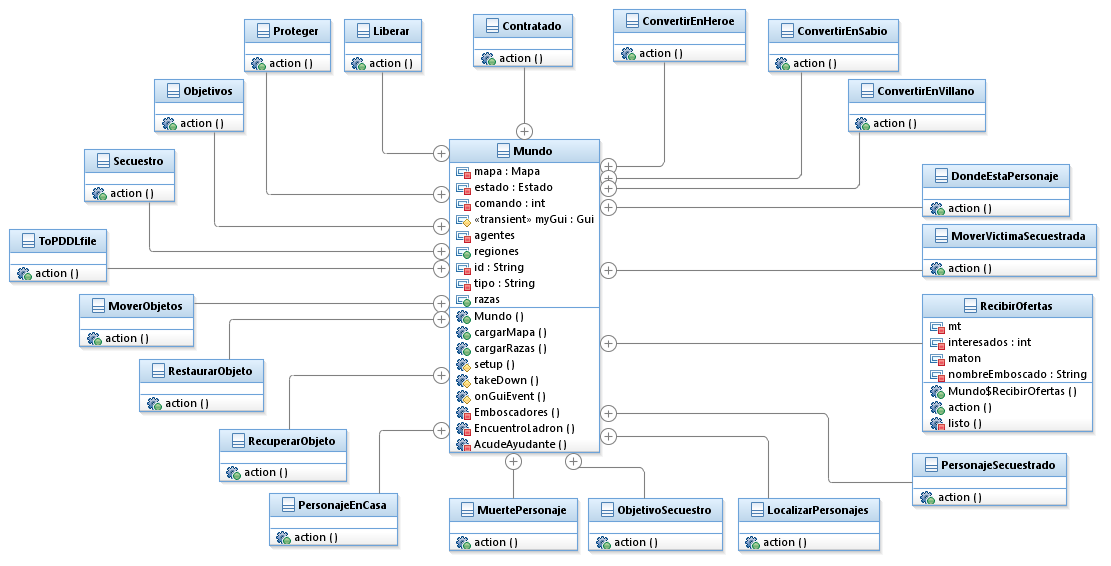
\includegraphics[width=0.9\textwidth]{Imagenes/ModelosGeneradorHistorias_DiagramaDeClaseMundo}
	\caption{Diagrama de Clase del Agente Mundo}
	\label{fig:DCMundo}
\end{figure}

\begin{figure}[h]
	\centering
	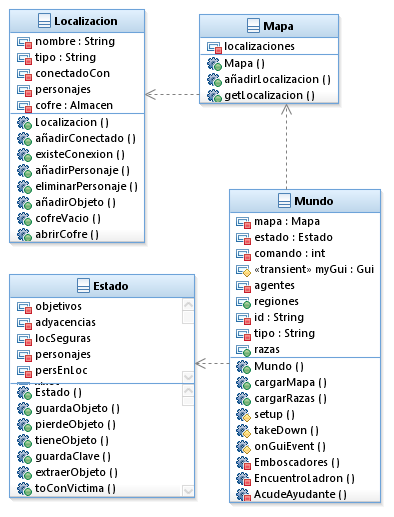
\includegraphics[width=0.9\textwidth]{Imagenes/ModelosGeneradorHistorias_DiagramaDeClaseMapa}
	\caption{Diagrama de Clase del Mapa}
	\label{fig:DCMapa}
\end{figure}

\begin{figure}[h]
	\centering
	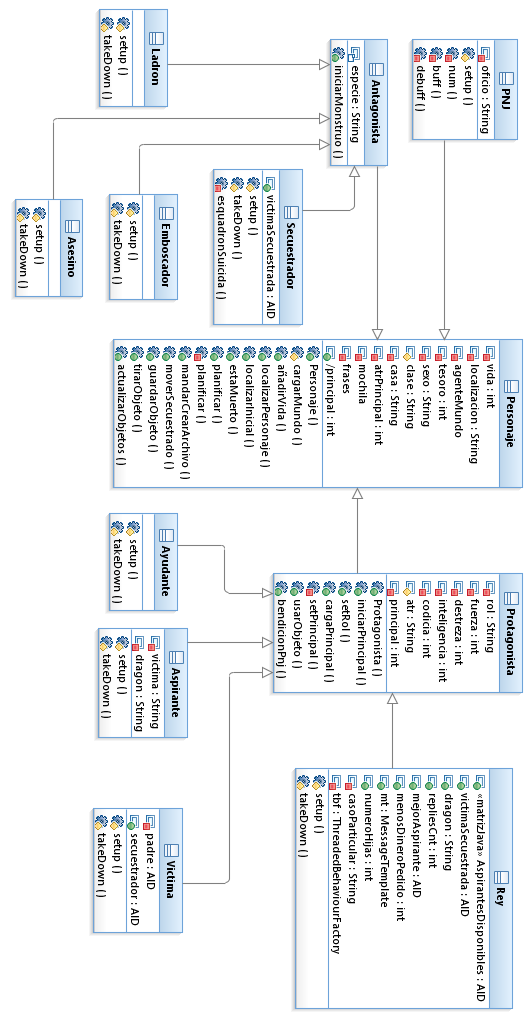
\includegraphics[width=0.9\textwidth]{Imagenes/ModelosGeneradorHistorias_DiagramaDeClasePersonajes}
	\caption{Diagrama de Clase de los Personajes}
	\label{fig:DCPersonajes}
\end{figure}

\begin{figure}[h]
	\centering
	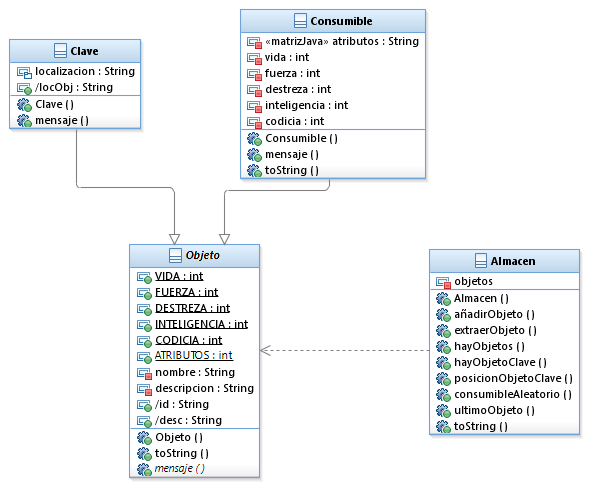
\includegraphics[width=0.9\textwidth]{Imagenes/ModelosGeneradorHistorias_DiagramaDeClaseObjetos}
	\caption{Diagrama de Clase de los Objetos}
	\label{fig:DCObjetos}
\end{figure}

\begin{figure}[h]
	\centering
	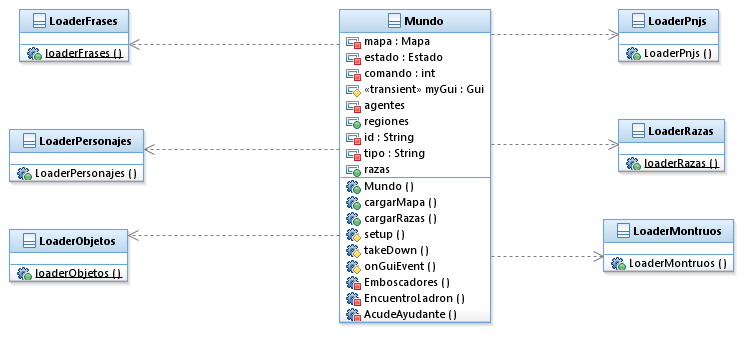
\includegraphics[width=0.9\textwidth]{Imagenes/ModelosGeneradorHistorias_DiagramaDeClaseLoaders}
	\caption{Diagrama de Clase de los SCD}
	\label{fig:DCLoaders}
\end{figure}

\begin{figure}[h]
	\centering
	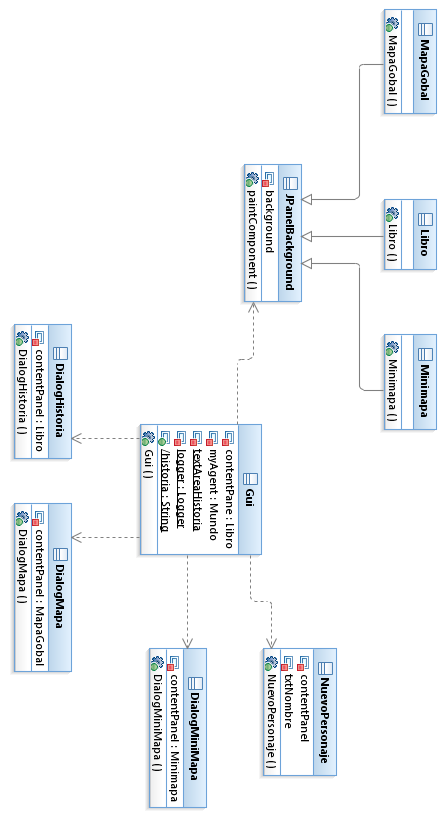
\includegraphics[width=0.9\textwidth]{Imagenes/ModelosGeneradorHistorias_DiagramaDeClaseGUI}
	\caption{Diagrama de Clase de la GUI}
	\label{fig:DCGUI}
\end{figure}